\subsection{Dijkstra's Algorithm}

The first solution proposed in this thesis is a modified version of Dijkstra's algorithm, which is a well-known algorithm for finding the shortest path between two vertices in a weighted graph. The algorithm works by selecting the node with the smallest distance from the source node and updating the distance of its neighbors. This process is repeated until all vertices have been visited. The algorithm is efficient for finding the shortest path between two vertices in a graph with non-negative edge weights. However, it is not suitable for graphs with negative edge weights.

Adapting the methodogies used by Pezzica et al. \cite{cormen2022introduction}, which incooperate the Dijkstra's algorithm with a (Minimum) Priority Queue data structure. The data structure maintains a dynamic set $S$ of elements, each set element in $S$ has a key and it supports the following dynamic-set operations.

\begin{itemize}
    \item INSERT($S; x; k$): inserts element $x$ with key $k$ into set $S$.
    \item MINIMUM($S$): returns element of $S$ with smallest key.
    \item EXTRACT-MIN($S$): removes and returns element of $S$ with smallest key.
    \item DECREASE-KEY($S;x;k$): decreases value of element $x$’s key to $k$. Assumes $k\leq x$’s current key value.
\end{itemize}

All operations take $O(\log n)$ time in an $n$-element heap with the exception of $\text{MINIMUM}(S)$ being $\Theta(1)$.

We extend the algorithm so that the algotithm will stop once all nodes within $t$ minutes have been visited. As the 15-Minute City concept is primarily used to study cities' characteristics, the input graph of the algorithm is expected to be far larger than each 15 minute area. Therefore, it is necessary to stop the algorithm once all nodes within $t$ minutes have been visited to prevent the algorithm from running indefinitely. The modified algorithm is shown in Algorithm \ref{alg:modified_dijsktra}.

\begin{algorithm}[H]
    \caption{Modified Dijkstra Algorithm} \label{alg:modified_dijsktra}
    \textbf{Input:} A graph $G(V,E)$, weights $w:E\rightarrow\mathbb{R}_{\geq 0}$, source vertex $s$, \\ \phantom{\textbf{Input:}} time threshold $t$ and $i$ denotes the index of the service type\\
    \textbf{Output} Assign $v.r[i]=1$ for vertices that can reach to source node $s$ within threshold $t$ % Set $S$ of vertices reachable by at most $t$ minutes
    \begin{algorithmic}
        \For {each vertex $v\in V$}
            \State $v.d\gets\infty$
        \EndFor
        \State $s.d\gets 0$
        % \State $S\gets\emptyset$
        \State $Q\gets\emptyset$
        \For {each vertex $v\in V$}
            \State INSERT($Q,v$)
        \EndFor
        \While {$Q\neq\emptyset$}
            \State $v\gets$EXTRACT-MIN$(Q)$
            \If {$v.d>t$}
                \State $Q\gets\emptyset$ \Comment{Break out of While loop}
            \Else
                % \State $S\gets S\cup\{v\}$
                \State $v.r[i] \gets 1 $
                \For {each vertex $u\in Adj[v]$}
                    \If {$u.d>v.d+w(u,v)$}
                        \State $u.d\gets v.d+w(u,v)$
                        \State DECREASE-KEY($Q,u,u.d$)
                    \EndIf
                \EndFor
            \EndIf
        \EndWhile
    \end{algorithmic}
\end{algorithm}

The modified Dijkstra's algorithm shown above only searches for vertices within $t$ minutes from a single source node. For our context of the 15-Minute City, this needs to run for each location of each service type. The full algorithm as the solution of the problem is shown in Algorithm \ref{alg:15mc}.

\begin{algorithm}[H]
    \caption{15-Minute City Algorithm}\label{alg:15mc}
    \textbf{Input:} A graph $G(V,E)$, weights $w:E\rightarrow\mathbb{R}_{\geq 0}$, a time threshold $t$ \\ \phantom{\textbf{Input:}} and a list $S$ of service vertices of $n$ types\\
    \textbf{Output} Set $R\subseteq V$ representing the $t$-Minute City
    \begin{algorithmic}
        \ForAll{vertex $v \in V$}
            \State $v.r \gets \{\mathbf{0}\}^{n}$
            \State $v.l \gets 0$
        \EndFor
        \ForAll{service $v \in S$}
            \State $v.l \gets i^{th}$ type of service
        \EndFor
        \For {each service type $i\in\{1,...,n\}$}
            % \State $S\gets\emptyset$
            \For {each vertex $s$ where $s.l=i$}
                \State $\text{Modified_Dijkstra}(G,w,s,t,i)$
                % \State $S\gets S\cup\text{ModifiedDijkstra}(G,w,s,t,i)$
            \EndFor
            % \For {each vertex $v\in S$}
            %     \State $v.r[i] \gets 1$
            % \EndFor
        \EndFor
        \State $R\gets\emptyset$
        \For {each vertex $v\in V$}
            \If {$v.r = \mathbf{1}$}
                \State $R \gets R\cup \{v\}$
            \EndIf
        \EndFor
    \end{algorithmic}
\end{algorithm}

\subsubsection{Analysis}

The time complexity of the modified Dijkstra's algorithm depends on the following:

\begin{itemize}
    \item Initialisation: $O(V)$
    \item $\text{INSERT}$: $|V|\cdot O(|\text{INSERT}|)=O(|V|\cdot|\text{INSERT}|)$
    \item $\text{EXTRACT-MIN}$: $|V|\cdot O(|\text{EXTRACT-MIN}|)=O(|V|\cdot|\text{EXTRACT-MIN}|)$
    \item $\text{DECREASE-KEY}$: $|E|\cdot O(|\text{DECREASE-KEY}|)=O(|E|\cdot|\text{DECREASE-KEY}|)$
\end{itemize}

The time complexity of the algorithm is also affected by the data structure used to implement the priority queue. A binary heap is a common choice for implementing a priority queue, which has a time complexity of $O(\log V)$ for $\text{INSERT}$, $\text{EXTRACT-MIN}$ and $\text{DECREASE-KEY}$ operations. However, if a Fibonacci heap is used instead, the time complexity of the operations is reduced to $O(1)$, $O(\log V)$ and $O(1)$ respectively.

As the latter two operations in the algorithm dominates the former two operations, the time complexity of algorithm \ref{alg:modified_dijsktra} is $O((V+E)\log V)$ if a binary heap is implemented. This can be reduced to $O(V\log V+E)$ if a Fibonacci heap is considered instead.

For the complete 15-Minute City Algorithm \ref{alg:15mc}, the algorithm is run for each location of each service type. Denote $m$ as the maximum number of locations for any service type, the time complexity of the algorithm is $O(n\cdot m\cdot(V\log V+E))$ if a binary heap is implemented and $O(n\cdot m\cdot(V\log V+E))$ if a Fibonacci heap is implemented. 

In both cases, the time complexity consider the size of the entire graph, which could be arbitrarily large when a city or a large area is studied. Due to the fact that the modified dijsktra's algorithm stops once all nodes within weight $t$ are searched, it is important to note that the actual complexity of the algorithm is much smaller. For example, consider a city with only square grids and each edge has a weight of 1 (see image \ref{fig:grid_city}) The algorithm will effectively only search a total of 100 edges and 141 nodes. In general, given a time threshold $t$, the number of nodes and edges searched by the modified dijastra algorithm can be calculated as follows:

$$|\text{Edges}|=4\cdot\sum^{t}_{l=1}(2t-1),\enspace|\text{Vertices}|=1+\sum^{t}_{l=1}4l$$

\begin{figure}[h]
    \caption{Example of grid city}
    \centering
    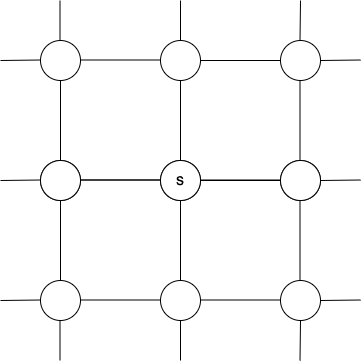
\includegraphics[width=0.5\textwidth]{grid_city.png}
    \label{fig:grid_city}
\end{figure}

However, if the graph of interest has the following characteristics: starting from the source node $s$, each node expands the graph with 4 edges of weight 1. (An illustration of the graph with 2 levels are shown in figure \ref{fig:tree_city}) In this arrangment, given a time threshold $t$ and $d$ the number of nodes branching out from each parent node, the number of nodes and edges can be calculated as follows:

$$|\text{Edges}|=\sum^{t}_{l=0}d^{l-1},\enspace|\text{Vertices}|=\sum^{t}_{l=1}d^{l-1}$$

This can be considered as the worst case for the algorithm. Setting $t=15$, the modified dijsktra's algorithm will have a time complexity with $|E|=357913941$ and $|V|=1431655765$.

\begin{figure}[h]
    \caption{Example of a tree city at 2 levels}
    \centering
    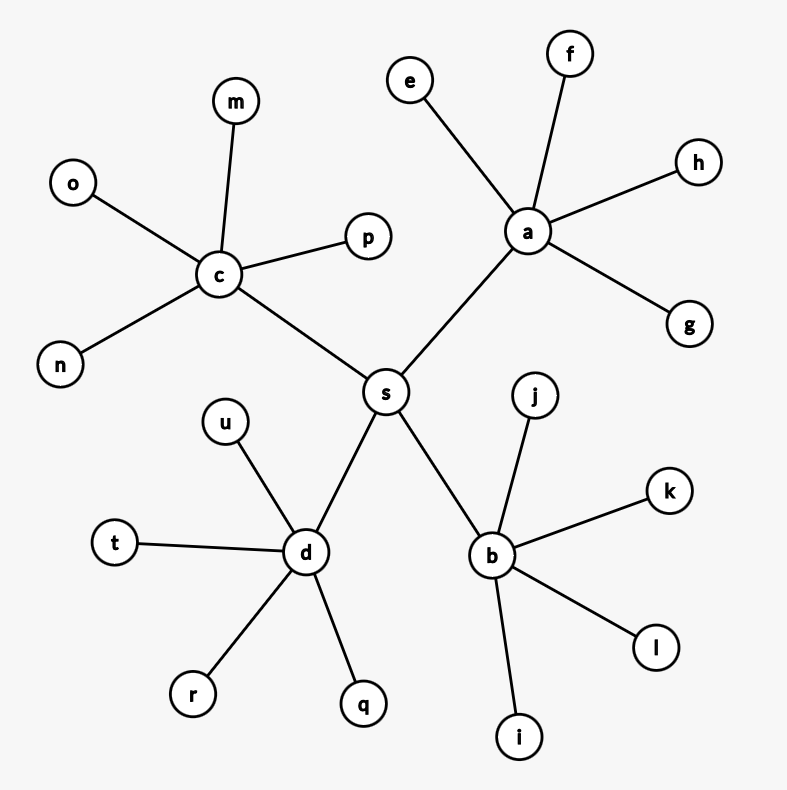
\includegraphics[width=0.5\textwidth]{tree_city.png}
    \label{fig:tree_city}
\end{figure}

\subsubsection{Drawbacks}

It is important to note that the proposed modification algorithm of Dijkstra's algorithm inserts all vertices of the graph into the priority queue set $Q$. In our tree city example shown above, the algorithm will insert all 1431655765 vertices into the set $Q$ and this is repeated for each service location of each type. Therefore, the algorithm proposed is not suitable for large graphs.

\subsection{Uniform Cost Search}

The problem described above can be solved by adapting a so-called "Uniform Cost Search" algorithm (also known as "Dijkstra for large graphs"). The algorithm is an extension of Best-first search and it is similar to Dijkstra's algorithm. However, Uniform Cost Search algorithm does not insert all vertices into the priority queue. Instead, it only inserts the vertices that are reachable within the time threshold $t$. A modification of this algorithm is shown in Algorithm \ref{alg:uniform_cost_search}. This algorithm can then be used in Algorithm \ref{alg:15mc} to replace the modified Dijkstra's algorithm in \ref{alg:modified_dijsktra}.

\begin{algorithm}[H]
    \caption{Modified_Uniform_Cost_Search} \label{alg:uniform_cost_search}
    \textbf{Input:} A graph $G(V,E)$, weights $w:E\rightarrow\mathbb{R}_{\geq 0}$, source vertex $s$, \\ \phantom{\textbf{Input:}} time threshold $t$ and $i$ denotes the index of the service type\\
    \textbf{Output} Assign $v.r[i]=1$ for vertices that can reach to source node $s$ within threshold $t$ % Set $S$ of vertices reachable by at most $t$ minutes
    \begin{algorithmic}
        \State $Q\gets\emptyset$ \Comment{Initialise an empty priority queue}
        % \State $R\gets\emptyset$ \Comment{Initialise a lookup table for reachable vertices}
        \State INSERT($Q,s$)
        \While {$Q\neq\emptyset$}
            \State $v\gets$EXTRACT-MIN$(Q)$
            \If {$v.d>t$}
                \State $Q\gets\emptyset$ \Comment{Break out of While loop}
            \Else
                \State $v.r[i] \gets 1 $
                \For {each vertex $u\in Adj[v]$}
                    \If {$u\notin Q$}
                        \State $u.d\gets v.d+w(u,v)$ % Update reached[u] to v.d+w(u,v)
                        \State INSERT($Q,u$)
                    \ElsIf{$u.d>v.d+w(u,v)$}
                        \State $u.d\gets v.d+w(u,v)$
                        \State DECREASE-KEY($Q,u,u.d$)
                    \EndIf
                \EndFor
            \EndIf
        \EndWhile
    \end{algorithmic}
\end{algorithm}

In this implementation, the time complexity remains the same as Dijkstra's algorithm in the worst case scenario. However, the algorithm is more efficient in practice as it only inserts vertices that are reachable within the time threshold $t$ into the priority queue. This reduces the number of vertices that need to be inserted into the priority queue.

\subsection{Inspirations from Johnson's algorithm}

Johnson's algorithm is an all-pairs shortest path algorithm to find shortest paths between every pair of nodes in a graph. It uses both Dijkstra and Bellman-Ford as subroutines and performs better than Floyd-Warshall algorithm in sparse graphs. For the goal of the 15-Minute City algorithm, the set of service vertices can be far smaller than the entire graph in size. Thus, all-pairs shortest path algorithms are not optimal solutions to the problem. However, Johnson's algorithm's approach in adjusting the weights to make all edges non-negative can be applied to the 15-Minute City problem. The algorithm works by adding a new vertex $s$ to the graph and adding edges from the new vertex to all vertices of the graph, before applying Bellman-Ford algorithm.

This approach can be applied to the 15-Minute City problem by adding a new vertex $s$ to the graph and adding edges from the new vertex to all service vertices of the same type. This would allow us to eliminate the inner loop of Algorithm \ref{alg:15mc} where $\text{ModifiedDijkstra}(G, w, s, t, i)$ is called. This alternate approach of the 15 Minute City algorithm is shown in Algorithm \ref{alg:15mc2}.

\begin{algorithm}[H]
    \caption{15-Minute City Algorithm} \label{alg:15mc2}
    \textbf{Input:} A graph $G(V,E)$, weights $w:E\rightarrow\mathbb{R}_{\geq 0}$, a time threshold $t$ \\ \phantom{\textbf{Input:}} and a list $S$ of service vertices of $n$ types\\
    \textbf{Output} Set $R\subseteq V$ representing the $t$-Minute City
    \begin{algorithmic}
        \ForAll{vertex $v \in V$}
            \State $v.r \gets \{\mathbf{0}\}^{n}$
            \State $v.l \gets 0$
        \EndFor
        \ForAll{service $v \in S$}
            \State $v.l \gets i^{th}$ type of service
        \EndFor
        \For {each service type $i\in\{1,...,n\}$}
            \State Create a new vertex $s$
            \State Add edges from $s$ to all vertices $v$ where $v.l=i$ and $w(s,v)=0$
            \State $\text{Modified_Uniform_Cost_Search}(G,w,s,t,i)$
            \State Remove $s$ and all edges connected  to it
        \EndFor
        \State $R\gets\emptyset$
        \For {each vertex $v\in V$}
            \If {$v.r = \mathbf{1}$}
                \State $R \gets R\cup \{v\}$
            \EndIf
        \EndFor
    \end{algorithmic}
\end{algorithm}